\chapter{Kubernetes: Insight and Auto-scaling}

\label{Chapter4} 

\section{Overview}

This chapter focus on the critical review and details setup of Kubernetes (k8s or Kube) cluster for deploying the auto-scalable ATHENA system. The Kubernetes key components are introduced, however, a more details and complete reference left it to the k8s official documentation\parencite{kubeDoc}.

With reference to the official website\footnote{\url{https://kubernetes.io}}, Kubernetes is the \emph{production grade container orchestration system that design for the deployment, scaling, management, and composition of application containers across clusters of hosts}. It is a robust container-management system that create a virtual abstraction layer on top of Cloud platform for deploying and maintaining scalable distributed systems. This abstraction enable users to deploy their applications consistently between different Cloud providers.

%Burns:2016:BOK:2898442.2898444

Kubernetes is the third incarnation of Google own container-management systems -- whereas the k8s is built upon its predecessors Borg and Omega \parencite{44843} systems over a decade experience of production run at scale. At Google with Borg system, \parencite{43438} reported that it \emph{runs hundreds of thousands of jobs, from many thousands of different applications, across a number of clusters each with up to tens of thousands of machines}\ldots

%In \parencite{Hightower:2017:KUR:3175917}, it claims that Google deploys over two billion application containers a week with Borg system. These figures are impressive but it comes in price. 

\section{Looking at Kubernetes Design}
\label{kubeDesign}
From Borg-Omega to Kubernetes, the Google software engineers learned lessons\parencite{44843} on how best to tackle with the container-management at design\footnote{\url{https://kubernetes.io/blog/2015/06/the-distributed-system-toolkit-patterns/}} and, bring the architecture to next level\footnote{\url{https://kubernetes.io/blog/2016/06/container-design-patterns/}} to make it easy for developers to write the distributed applications and services that run in cloud and datacenter environments. Looking at Kubernetes, we can observe that the design of the system become more generic and abstraction compare to its predecessors. It goes beyond more than container-management. Since the process of containerisation encapsulates the application, Kubernetes introduces \textit{Application-Oriented Infrastructure} (AOI) with two motivations:
\begin{itemize}
\item abstracting away details of machine and operating system from application developer and deployment
\item \emph{single application process per container} Design Pattern entails that managing containers mean managing applications, therefore, it shifts the Kube API from machine-oriented to application-oriented and, improves application deployment and introspection 
\end{itemize}

\noindent\textbf{Objects Management:} \quad To model a generalised system is a challenging goal for every distributed system designer. To realise this generalisation, at very abstract, Kubernetes is just a \textbf{Objects Management} API service. The Kubernetes API does not perform the functional aspect of the system, but the objects its managed deliver these functionality. In Kubernetes, we can define the type of what kind, which does something. The shape of the Kubernetes Object can be expressed in YAML format. The mandatory fields for a Kubernetes Object are summarised in Table~\ref{kubeObjectTable}.

\begin{table}[H]
\centering
    \begin{tabular}{ | l | p{11cm} |}
    \hline
    Field & Description \\ \hline
    apiVersion & Which version of the Kubernetes API using to create this object. \\ \hline
    kind & What kind of object you want to create. \\ \hline
    metadata & Data that helps uniquely identify the object, including a name string, UID, and optional namespace. \\ \hline
    spec & To Describe the desired state of the object. Precise format of the object spec is different for every Kubernetes object, and contains nested fields specific to that object. \\ \hline
    status & Provides read-only information about the current state of the object, is supplied and updated by the Kubernetes system. Like spec, format is vary by object type. \\
    \hline
    \end{tabular}
\caption{Kubernetes Object Mandatory Fields}
\label{kubeObjectTable}
\end{table}

\noindent\textbf{Work Out:} \quad To understand how Objects Management work in Kubernetes API, we will go through a quick exercise. Consider we have Kubernetes and its API service up and running. Consider we like to create an object of type, say, \ctexttt{FireBall}. Create a YAML as follows.

\begin{lcverbatim}
apiVersion: apiextensions.k8s.io/v1beta1
kind: CustomResourceDefinition
metadata:
  name: fireballs.api.sankholin.com
spec:
  group: api.sankholin.com
  version: v1
  scope: Namespaced
  names:
    plural: fireballs
    singular: fireball
    kind: FireBall
\end{lcverbatim}

\noindent And create this \ctexttt{FireBall} type in Kube API:
\begin{lcverbatim}
kubectl create -f CRD_Fireball.yaml
kubectl get crd
kubectl api-versions
\end{lcverbatim}

\noindent And now we can prescribe our \ctexttt{FireBall} type in YAML as follows. Notice of \emph{kind} field.

\begin{lcverbatim}
apiVersion: "api.sankholin.com/v1"
kind: FireBall
metadata:
  name: my-fireball-object
spec:
  image: sankholin.com/fireball-container-image:latest
\end{lcverbatim}

\noindent Finally, create an instance of \ctexttt{FireBall} custom Kubernetes object.
\begin{lcverbatim}
kubectl create -f my-fireball.yaml
kubectl get fireball
kubectl get fireball -o yaml
\end{lcverbatim}

\noindent Note that \verb|my-fireball-object| custom object contains custom field \verb|spec.image|, which can be arbitrary JSON field and, for example, this will pull and deploy the containerised \emph{FireBall} application image from \emph{Container Image Registry}. The use of \textit{FireBall} nomenclature is intentional and the exact behaviour of what \emph{FireBall} type might do is left it for reader interpretation -- e.g. a cluster of Game engine. This is to show that how Kube API handle custom resources in a generic way through \ctexttt{CustomResourceDefinition}. Kube Objects are persistent entities (i.e. CRUD\footnote{Create, Read, Update, Delete}) which represent the state of the cluster. In this exercise, we are using \ctexttt{CustomResourceDefinition} which is one of the built-in resource type of Kube API which purpose is to be able to create a \textit{Custom Resources} inside Kube system. Table~\ref{kubeBuiltinResources} summarise the commonly use Kubernetes built-in Resources\footnote{Resource as in RESTful architecture} (or \emph{kind}).

\begin{table}[H]
\centering
    \begin{tabular}{ | l | p{12cm} |}
    \hline
    Kind & Description \\ \hline
    \href{https://kubernetes.io/docs/concepts/workloads/pods/pod-overview/}{Pod} & The basic building block of Kubernetes -- the smallest and simplest unit in the Kubernetes object model. \\ \hline
    \href{https://kubernetes.io/docs/concepts/services-networking/service/}{Service} & Service is an abstraction which defines a logical set of Pods and a policy by which to access them - sometimes called a micro-service. \\ \hline
    \href{https://kubernetes.io/docs/concepts/workloads/controllers/replicaset/}{ReplicaSet} & Next-generation Replication Controller. A ReplicaSet ensures that a specified number of pod replicas are running at any given time. \\ \hline
    \href{https://kubernetes.io/docs/concepts/workloads/controllers/deployment/}{Deployment} & Deployment controller provides declarative updates for Pods and ReplicaSets. You describe a desired state in a Deployment object, and the Deployment controller changes the actual state to the desired state at a controlled rate. \\ \hline
    \href{https://kubernetes.io/docs/concepts/workloads/controllers/statefulset/}{StatefulSets} & StatefulSet is the workload API object used to manage stateful applications. \\ \hline
    \href{https://kubernetes.io/docs/concepts/workloads/controllers/daemonset/}{DaemonSet} & A DaemonSet ensures that all (or some) Nodes run a copy of a Pod. As nodes are added to the cluster, Pods are added to them. As nodes are removed from the cluster, those Pods are garbage collected. \\ \hline
    \href{https://kubernetes.io/docs/concepts/workloads/controllers/jobs-run-to-completion/}{Job} & A job creates one or more pods and ensures that a specified number of them successfully terminate. \\ \hline
    \href{https://kubernetes.io/docs/concepts/workloads/controllers/cron-jobs/}{CronJob} & A Cron Job manages time based Jobs, run: Once or Repeatedly at a specified point in time. \\
    \hline
    \end{tabular}
\caption{Kubernetes Built-in Resources}
\label{kubeBuiltinResources}
\end{table}

Note that Table~\ref{kubeBuiltinResources} is just introductory Kubernetes resources that need to get started work on with the Kubernetes in most use cases. For the interest of thesis length, it is recommended to read Kubernetes documentation \parencite{kubeDoc} for how these built-in Kubernetes resources work in specific to their functionality.

\section{Tackling at Production Ready Setup}

Kubernetes is a much more complex system to up and run with -- it is quite a daunting task for setting up \emph{Production Ready} Kubernetes deployment for user's own on-premise, bare-metal or Private Cloud infrastructure. It has steep learning curve. Its breadth of functionality grows daily, documentation is outdated quickly and is enough to overwhelm even the most advanced users. Every layer of Kubernetes have a couple of different ways to setup and options to pick. Nevertheless, Kubernetes composes of components for \textbf{Master} role and components for the \textbf{Node} role. Table~\ref{kubeMasterComp} and Table~\ref{kubeNodeComp} summarise this. These components are fundamental executables for up and running the Kubernetes cluster. 

\begin{table}[H]
\centering
    \begin{tabular}{ | l | p{10cm} |}
    \hline
    Component & Description \\ \hline
    \href{https://kubernetes.io/docs/reference/command-line-tools-reference/kube-apiserver/}{kube-apiserver} & exposes the API and the front-end for the Kubernetes control plane \\ \hline
    \href{https://kubernetes.io/docs/reference/command-line-tools-reference/kube-scheduler/}{kube-scheduler} & monitor newly created pods and selects a node for them to run on \\ \hline
    \href{https://kubernetes.io/docs/reference/command-line-tools-reference/kube-controller-manager/}{kube-controller-manager} & control loop that watches the shared state of the cluster through the apiserver and makes changes attempting to move the current state towards the desired state \\ \hline
    \href{https://kubernetes.io/docs/tasks/administer-cluster/configure-upgrade-etcd/}{etcd} & consistent and highly-available key value store backing for all cluster data \\
    \hline
    \end{tabular}
\caption{Components for Kubernetes Master Role}
\label{kubeMasterComp}
\end{table}

\noindent \textbf{Hard Way:} \quad For straight forward approach, we could spin up one node and install all the components mention in Table~\ref{kubeMasterComp} to run as Kube Master role. And spin up one or more nodes to install all the components mention in Table~\ref{kubeNodeComp} to run as Kube Node role. Since Kubernetes is written in GoLang\footnote{\url{https://golang.org}}, we could download the source -- compile, build -- or, download pre-compiled binary and run executables in foreground or, wrap into \verb|systemd| daemon services. This would work in principle, at least. However so, this has to deal with more low level handling and, generally \emph{"goto"} setup for a Kube developer.

\begin{table}[H]
\centering
    \begin{tabular}{ | l | p{11cm} |}
    \hline
    Component & Description \\ \hline
    \href{https://kubernetes.io/docs/reference/command-line-tools-reference/kubelet/}{kubelet} & An agent that runs on each node in the cluster. It makes sure that containers are running in a pod. \\ \hline
    \href{https://kubernetes.io/docs/reference/command-line-tools-reference/kube-proxy/}{kube-proxy} & enables the Kubernetes service abstraction by maintaining network rules on the host and performing connection forwarding \\  \hline
    container-runtime & the software that is responsible for running containers -- supports several runtimes: \textbf{Docker}, \textbf{rkt}, \textbf{runc} and any Open Container Initiative (OCI) runtime specification implementation \\
    \hline
    \end{tabular}
\caption{Components for Kubernetes Node Role}
\label{kubeNodeComp}  
\end{table}

\noindent \textbf{Streamline Toolkit:} \quad Up and running in \emph{Hard Way} is not an ideal for \emph{Production Ready} setup. For this purpose, Kube community has diverse range of streamline solution for many different setup that are specifics to Public Cloud Provider, Linux distro, and so on. Table~\ref{kubeToolkits} summarise the recommended toolkit selection for setting up Kube cluster. 

\begin{table}[H]
\centering
    \begin{tabular}{ | l | p{12cm} |}
    \hline
    Toolkit & Description \\ \hline
    \href{https://kubernetes.io/docs/setup/independent/create-cluster-kubeadm/}{kubeadm} & bootstrap a best-practice Kubernetes cluster in an easy, reasonably secure and extensible way. \textbf{Kubernetes Certified}. \\ \hline
    \href{https://github.com/kubernetes-incubator/kubespray}{Kubespray} & install a Kubernetes cluster hosted on GCE, Azure, OpenStack, AWS, or Baremetal. Ansible. \\  \hline
    \href{https://github.com/kubernetes/kops}{kops} & helps you create, destroy, upgrade and maintain production-grade, highly available, Kubernetes clusters from the command line for AWS \\
    \hline
    \end{tabular}
\caption{Toolkits for Streamline Kubernetes Cluster Setup as of v1.10}
\label{kubeToolkits}
\end{table}

The kubeadm is chosen to bootstrap the Kube cluster for the purpose of ATHENA deployment. However, also note that, Kubernetes documentation offer dozens of different ways\footnote{\url{https://kubernetes.io/docs/setup/pick-right-solution/}} to setup Kube cluster. This research finds that \textbf{kubeadm} is the most appropriate toolkit for setting up \emph{Production Ready} Kubernetes cluster. The justification for \emph{why kubeadm} is because it is the Kubernetes \textbf{Certified Solution} as of v1.10, its abstraction to IaC automation tool and it can streamline the upgrade of the Kube cluster reliably well as shown below.

\begin{small}
\begin{lcverbatim}
root@athena-kube-master1:~# kubeadm upgrade plan
[preflight] Running pre-flight checks.
[upgrade] Making sure the cluster is healthy:
(scrap)
Components that must be upgraded manually after you have upgraded the \
   control plane with 'kubeadm upgrade apply':
COMPONENT   CURRENT      AVAILABLE
Kubelet     4 x v1.9.4   v1.10.2

Upgrade to the latest stable version:
COMPONENT            CURRENT   AVAILABLE
API Server           v1.9.4    v1.10.2
Controller Manager   v1.9.4    v1.10.2
Scheduler            v1.9.4    v1.10.2
Kube Proxy           v1.9.4    v1.10.2
Kube DNS             1.14.7    1.14.7
Etcd                 3.1.11    3.1.11

You can now apply the upgrade by executing the following command:
	kubeadm upgrade apply v1.10.2
Note: Before you can perform this upgrade, you have to update kubeadm to v1.10.2.

_____________________________________________________________________

root@athena-kube-master1:~# apt-get install --only-upgrade kubeadm
(scrap)
root@athena-kube-master1:~# kubeadm upgrade apply v1.10.2
(scrap)
\end{lcverbatim}
\end{small}

\noindent Figure~\ref{fig:kubeadm} shows the result of Kubernetes components installed into Master and Node role respectively using kubeadm. 

\begin{figure}[H]
\centering
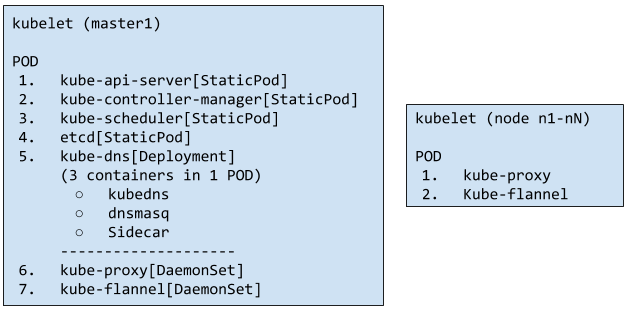
\includegraphics[width=0.55\paperwidth]{Figures/KUBE_kubeadm}
\decoRule
\caption[Kubernetes components on Master and Node using kubeadm]{Kubernetes components on Master and Node using kubeadm}
\label{fig:kubeadm}
\end{figure}

\noindent It is interesting to observe that at the basic bootstrapping for \textbf{a Kube Node} means a machine installed with \textbf{just kubelet component and container runtime engine}. After kubelet and Docker container runtime engine installed, up and and running as a \verb|systemd| daemon service, a Pod can be deployed. Therefore, Figure~\ref{fig:kubeadm} shows that api-server, controller-manager, scheduler, etcd components are running as Pods on a node with Master role; and similarly kube-proxy is running as Pod on both Master and Node roles.

Recall Table~\ref{kubeBuiltinResources} that a Pod is the built-in resource type (a \emph{kind}) and the basic unit of Kubernetes Object model. In this case, the kube-api-server, a GoLang application is containerised and deployed as a Pod. The \verb|kube-apiserver.yaml| manifests as follows.

\begin{lcverbatim}
apiVersion: v1
kind: Pod
metadata:
  labels:
    component: kube-apiserver
    tier: control-plane
  name: kube-apiserver
  namespace: kube-system
spec:
  containers:
  - command:
    - kube-apiserver
    image: gcr.io/google_containers/kube-apiserver-amd64:v1.10.2
    (scrap)
\end{lcverbatim}

However, note that, kubeadm created the kube-apiserver component as a special Pod type called Static Pod. From k8s documentation\footnote{\url{https://kubernetes.io/docs/tasks/administer-cluster/static-pod/}}, \parencite{kubeDoc} states that \emph{Static Pods are managed directly by kubelet daemon on a specific node, without the API server observing it. Kubelet automatically creates so-called mirror pod on the Kubernetes API server for each static pod, so the pods are visible there, but they cannot be controlled from the API server}. From this, we can also observe that kubelet can directly bootstrap a Pod, and it shares the Kubernetes objects management along with the kube-apiserver to sudden extent.

\subsection{Add-ons}

In addition to the Kubernetes Master and Node components (Tables~\ref{kubeMasterComp}, \ref{kubeNodeComp}), we can also observe that there are kube-dns on Master role (installed by part of \verb|kubeadm init|\footnote{\url{https://kubernetes.io/docs/reference/setup-tools/kubeadm/kubeadm-init/}}) and, kube-flannel running on both Master and Node role. These components are called \textbf{Add-ons}\footnote{\url{https://kubernetes.io/docs/concepts/cluster-administration/addons/}} which extend the functionality of Kubernetes. Table~\ref{kubeadmAddons} summarise components that are deployed as part of the bootstrapping Kubernetes cluster.

\begin{table}[H]
\centering
    \begin{tabular}{ | l | p{11cm} |}
    \hline
    Add-ons & Description \\ \hline
    \href{https://github.com/kubernetes/kubernetes/tree/master/cluster/addons/dns/kube-dns}{kube-dns} & The internal implementation for Kubernetes DNS service. \\ \hline
   \href{https://github.com/coreos/flannel}{kube-flannel} & Flannel is an overlay network provider that can be used with Kubernetes Pod network. \\ 
    \hline
    \end{tabular}
\caption{Additional compulsory Kubernetes add-ons components}
\label{kubeadmAddons}  
\end{table}

\noindent To bootstrap the full-fledge \emph{Production Ready} Kubernetes cluster, there are compulsory add-ons such as like these. Note though that, Kubernetes documentation \parencite{kubeDoc} offer dozens of Add-ons; some of which are competing technologies and alternatives for the particular functionality e.g. to use \textbf{Weave Net} instead of \textbf{Flannel} for Pod Networking.

\subsection{Pod Networking}

From Table~\ref{kubeadmAddons}, there is a notion of \textbf{Overlay Network}. In Kubernetes, the concept of Pod is to encapsulates containers. A Kube Pod object holds one or more containers and, introduces \textbf{IP-per-Pod} for network model. It implies IP addressing at the Pod scope. Therefore, containers within a Pod share their network namespaces including their IP address. The Pod networking requirement \parencite{kubeDoc} states that nodes and containers can communicate each others without Network Address Translation (NAT). Therefore, the IP that a container sees itself as is the same IP that others see it as. In a nutshell, Kubernetes network model imposes barring usage of intentional network segmentation policies such as NAT. Kubernetes documentation offers dozens of different ways\footnote{\url{https://kubernetes.io/docs/concepts/cluster-administration/networking/}} for implementing this networking requirement -- Overlay Network is one of them. The implementation usually offer as \emph{Add-ons}, however, it is a compulsory step. Medium articles by google-cloud\footnote{\url{https://medium.com/google-cloud/understanding-kubernetes-networking-pods-7117dd28727}}, ApsOps\footnote{\url{https://medium.com/@ApsOps/an-illustrated-guide-to-kubernetes-networking-part-2-13fdc6c4e24c}} illustrated details on how Overlay Network is used for Kubernetes Pod networking requirement. %It is observed that with Overlay Network, Kubernetes cluster can be extended across multiple Cloud providers and geographically separated data centres.

For the context of \emph{compute auto-scaling research} presenting in this thesis, the further investigation on performance comparison of Pod Networking with competing technologies left out for future work.

\subsection{Service}
\label{kubeService}
\noindent \textbf{Service Proxies:} \quad In Kubernetes, Pods are ephemeral and mortal. This is due to the fact that the Kube cluster can replicate Pod (destroy and re-create new) for dynamically scale up or down, self-healing and self-managing purposes. As the Pod get destroyed or recycled, the Pod IP address may change. This is not the desire effect for the application developer to keep track of these IP addresses. Service is an network abstraction layer to retain the consistent endpoint within the cluster. Service can be also seen as frontend service proxies for other Kubernetes objects such as Pod, Deployment, ReplicaSet, etc. For the implementation, kube-proxy is responsible for creating a form of Virtual IP in 3 different proxy modes -- userspace, iptables, IPVS --  for Services of type other than ExternalName. For publishing services, it offers 4 different types as summarise in Table~\ref{kubeServiceTypes}.

\begin{table}[H]
\centering
    \begin{tabular}{ | l | p{11cm} |}
    \hline
    Type & Description \\ \hline
    ClusterIP & Exposes the service on a cluster-internal IP. \textbf{Default type}. \\ \hline
    NodePort & Exposes the service on each Node’s IP at a static port. \\  \hline
    LoadBalancer & Exposes the service externally using a cloud provider’s load balancer. \\ \hline
    ExternalName & Maps the service to the contents of the externalName field (e.g. foo.bar.example.com), by returning a CNAME record with its value. \\
    \hline
    \end{tabular}
\caption{Kubernetes service types for publishing service endpoints}
\label{kubeServiceTypes}  
\end{table}

\noindent \textbf{Service Discovery:} \quad For Service Discovery purpose, Kubernetes runs internal DNS. This comes in as Add-ons, however, compulsory. Kubeadm deployed kube-dns\footnote{\url{https://kubernetes.io/docs/tasks/administer-cluster/dns-custom-nameservers/}} Pod for this purpose. For example, the following \verb|athena-ui.yaml| service manifest creates a service endpoint for the athena-ui.

\begin{small}
\begin{lcverbatim}
apiVersion: v1
kind: Service
metadata:
  labels:
    app: athena-ui
  name: athena-ui
spec:
  ports:
    - port: 80
  selector:
    app: athena-ui
\end{lcverbatim}
\end{small}

\noindent The following screenshot shows ATHENA's components and their service proxies setup. 

\begin{small}
\begin{lcverbatim}
root@athena-kube-master1:~# kubectl get svc
NAME                TYPE        CLUSTER-IP       EXTERNAL-IP   PORT(S)   AGE
athena-analytics    ClusterIP   10.103.197.212   <none>        80/TCP    61d
athena-api-server   ClusterIP   10.101.72.108    <none>        80/TCP    54d
athena-ui           ClusterIP   10.103.117.69    <none>        80/TCP    82d
\end{lcverbatim}
\end{small}

\noindent In this example, we can say that, the \verb|athena-ui.yaml| service manifest created a DNS
\\
\verb|athena-ui.default.svc.cluster.local|
\\
that resolve to the Service Endpoint IP address \verb|10.103.117.69|.
\\
\\
\noindent \textbf{Exposing Service Endpoint:} \quad We can reach to the service's \textbf{ClusterIP}, from all nodes within cluster, e.g:

\begin{small}
\begin{lcverbatim}
root@athena-kube-master1:~# curl -s --user (scrap):(scrap) 10.101.72.108/api/version
{"version":"1.0.1-SNAPSHOT"}
root@athena-kube-n1:~# curl -s --user (scrap):(scrap) 10.101.72.108/api/version
{"version":"1.0.1-SNAPSHOT"}
root@athena-kube-n2:~# curl -s --user (scrap):(scrap) 10.101.72.108/api/version
{"version":"1.0.1-SNAPSHOT"}
root@athena-kube-n3:~# curl -s --user (scrap):(scrap) 10.101.72.108/api/version
{"version":"1.0.1-SNAPSHOT"}
\end{lcverbatim}
\end{small}

\noindent Kubernetes offers few different possibilities -- \textbf{NodePort, LoadBalancer, HostNetwork, HostPort, Ingress} -- to expose the service endpoint to outside world, i.e. Public network. For production setup, cloude provider's LoadBalancer or Ingress\footnote{\url{https://kubernetes.io/docs/concepts/services-networking/ingress/}} should be used, however, on NeCTAR, every VM instances get Public IP address. In this case, setting up a simple HAProxy \textbf{Layer-4/Layer-7} routing deliver the similar effect.

\begin{small}
\begin{lcverbatim}
root@athena-kube-n1:~# ip a|grep eth0|grep inet
    inet 115.146.85.147/22 brd 115.146.87.255 scope global eth0

root@athena-kube-n1:~# tail -6 /etc/haproxy/haproxy.cfg
frontend loadbalancer
	bind *:80
	default_backend athena

backend athena
	server api1 10.101.72.108
\end{lcverbatim}
\end{small}

\subsection{Volume and Storage}

Kubernetes also offer dozens of different ways\footnote{\url{https://kubernetes.io/docs/concepts/storage/volumes/}} for setting up volume and storage. Likewise in Docker container, volume in Kubernetes are ephemeral i.e. data will be lost if the Pod restart has happened. Table~\ref{kubeVol} list some basic volume that can be used by Kubernetes Pod, StatefulSets, etc.

\begin{table}[H]
\centering
    \begin{tabular}{ | l | p{11cm} |}
    \hline
    Type & Description \\ \hline
    emptyDir & An emptyDir volume is first created when a Pod is assigned to a Node, and exists as long as that Pod is running on that node. \\ \hline
    hostPath & A hostPath volume mounts a file or directory from the host node’s filesystem into your Pod. \\  \hline
    nfs & An nfs volume allows an existing NFS (Network File System) share to be mounted into your Pod. \\
    \hline
    \end{tabular}
\caption{Kubernetes basic volume storage}
\label{kubeVol}  
\end{table}

\noindent The production setup should explore a better solution space in cluster file system such as setting up generic GlusterFS, CephFS, or cloud provider specific OpenStack Cinder, AWS ElasticBlockStore or a more performance iSCSI, Fibre Channel, and parallel distributed clustered file system such as IBM GPFS or LustreFS.

For the context of \emph{compute auto-scaling research} presenting in this thesis, the further investigation on scaling of volume and data storage left out for future work.

\section{Instrumentation and Metrics}
\label{metrics}
Kubernetes core components (Tables~\ref{kubeMasterComp}, \ref{kubeNodeComp}) are instrumented and exposed at \verb|/metrics|. By default, metrics are in Prometheus format\footnote{\url{https://prometheus.io/docs/instrumenting/exposition_formats/}}. When making HTTP GET request to \verb|/metrics| on the component being monitored, it expects to return a set of line delimited metrics. The following is an example of kube-apiserver component metrics.

\begin{small}
\begin{lcverbatim}
curl -s 127.0.0.1:8001/metrics | grep process_cpu_seconds_total
# HELP process_cpu_seconds_total Total user and system CPU time spent in seconds.
# TYPE process_cpu_seconds_total counter
process_cpu_seconds_total 167305.1
\end{lcverbatim}
\end{small}

\noindent Among these core components, kubelet is one of the most important components in Kubernetes. Kubelet makes sure containers run inside Pod, runs container probe and, reports the status back to the kube-apiserver. Kubelet also comes with an embedded cAdvisor\footnote{\url{https://github.com/google/cadvisor}} instance which collects, aggregates, processes and exports metrics such as CPU, memory and network usage of running containers. Kubelet exposes cAdvisor metrics at \verb|/metrics/cadvisor|. 

\begin{small}
\begin{lcverbatim}
curl -s 127.0.0.1:10255/metrics/cadvisor|grep container_cpu_usage_seconds_total
container_cpu_usage_seconds_total{container_name="athena-worker", (scrap)"} 218.975
\end{lcverbatim}
\end{small}

\noindent \textbf{Kubelet Summary API} also expose aggregated node and Pods metrics as follows.

\begin{small}
\begin{lcverbatim}
curl -s http://localhost:10255/stats/summary | less
{ "node": {
   "nodeName": "athena-kube-n3",
   "systemContainers": [
    {
     "name": "runtime",
     "startTime": "2018-06-07T06:51:55Z",
     "cpu": {
      "time": "2018-06-09T13:47:57Z",
      "usageNanoCores": 39373255,
      "usageCoreNanoSeconds": 79051470783486
     },
     "memory": {
      "time": "2018-06-09T13:47:57Z",
      "usageBytes": 5535948800,
      "workingSetBytes": 1090809856,
      "rssBytes": 103976960,
      "pageFaults": 18562442,
      "majorPageFaults": 558
     },
    (scrap)
\end{lcverbatim}
\end{small}

Before Kubernetes v1.9, the popular stack is Heapster + InfluxDB for consuming these metrics and storing them as timeseries data. However, as of v1.10, Heapster is deprecated\footnote{\url{https://github.com/kubernetes/heapster/blob/master/docs/deprecation.md}} in favour for an overhaul with Metrics API\footnote{\url{https://brancz.com/2018/01/05/prometheus-vs-heapster-vs-kubernetes-metrics-apis/}} at Kubernetes Instrumentation and monitoring architecture\footnote{\url{https://github.com/kubernetes/community/blob/master/contributors/design-proposals/instrumentation/monitoring_architecture.md}}. And the Metrics Server is the official\footnote{\url{https://kubernetes.io/docs/tasks/debug-application-cluster/core-metrics-pipeline/}} successor to replace Heapster. Prometheus is used for the monitoring and scraping various Kubernetes components metrics. In particular, \textbf{Prometheus Operator\footnote{\url{https://github.com/coreos/prometheus-operator}} + kube-prometheus\footnote{\url{https://github.com/coreos/prometheus-operator/tree/master/contrib/kube-prometheus}}} stack  is chosen empirically based on different trials. Prometheus is primarily a pull style monitoring platform. The justification for \textit{why Prometheus} is mainly based on this metrics polling approach for better performance outcome. This essentially does not impose stress and load on the monitored application. Furthermore, Prometheus offer many third-party metrics exporters\footnote{\url{https://prometheus.io/docs/instrumenting/exporters/}} such as the JMX exporter which can export from a wide variety of JVM-based applications (e.g. ActiveMQ, Kafka) and, timing and gauging HTTP Requests/Responses (e.g. Apache, Nginx, HAProxy) metrics and workload.
%\begin{figure}[H]
%\centering
%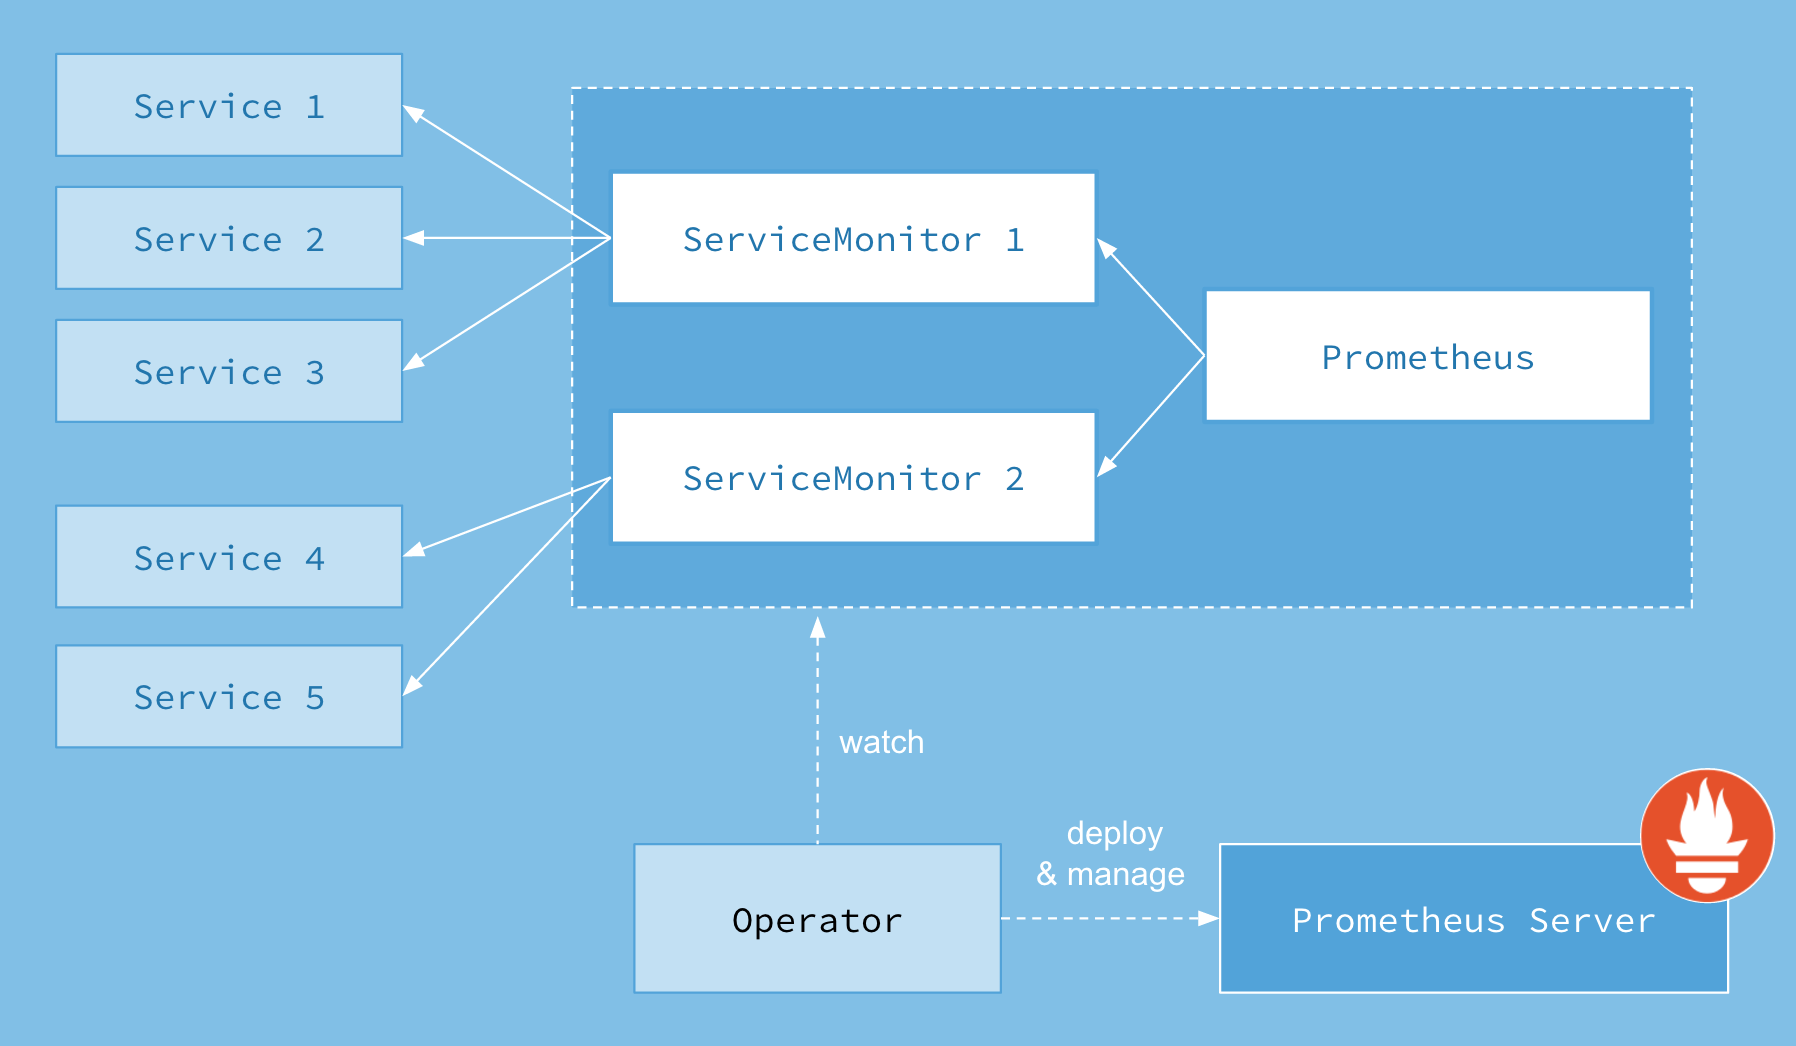
\includegraphics[width=0.5\paperwidth]{Figures/Prom_Operator_Architecture}
%\decoRule
%\caption[Prometheus]{Prometheus Operator Architecture}
%\label{fig:promOpsArch}
%\end{figure}
%*Prometheus Operator Architecture image taken from https://coreos.com/operators/prometheus/docs/latest/user-guides/getting-started.html
%\newpage
\\
\\
\noindent \textbf{Prometheus Operator:} \quad It\footnote{\url{https://coreos.com/operators/prometheus/docs/latest/user-guides/getting-started.html}} creates, configures, and manages Prometheus monitoring instances and, introduces "monitoring" namespace and additional resources Alertmanager and ServiceMonitor to Kubernetes API through \ctexttt{CustomResourceDefinition} (section~\ref{kubeDesign}). The ServiceMonitor uses Kube's Label and Selector to intercept Kubernetes Services (section \ref{kubeService}) and their exposed Prometheus format metrics (i.e. \verb|/metrics|) in evasive way.

\begin{small}
\begin{lcverbatim}
root@athena-kube-master1:~# kubectl get crd
NAME                                    AGE
alertmanagers.monitoring.coreos.com     20d
prometheuses.monitoring.coreos.com      20d
servicemonitors.monitoring.coreos.com   20d
root@athena-kube-master1:~# kubectl get namespaces
NAME          STATUS    AGE
monitoring    Active    20d
root@athena-kube-master1:~# kubectl api-versions|grep monitoring
monitoring.coreos.com/v1
\end{lcverbatim}
\end{small}

\noindent \textbf{Monitoring Setup:} \quad The Metrics Server (Heapster replacement) setup is straight forward. We can create it from the provided manifests as follows.

\begin{small}
\begin{lcverbatim}
root@athena-kube-master1:~# git clone \
		https://github.com/kubernetes-incubator/metrics-server.git
(scrap)
root@athena-kube-master1:~# cd metrics-server
root@athena-kube-master1:~/metrics-server# kubectl create -f deploy/1.8+/
(scrap)
\end{lcverbatim}
\end{small}

Once Metrics Server is up and running, we can observe the cluster wide metrics and monitoring that is scraped from Kubelet Summary API.

\begin{small}
\begin{lcverbatim}
root@athena-kube-master1:~# kubectl api-versions|grep metrics
metrics.k8s.io/v1beta1
root@athena-kube-master1:~# kubectl top node
NAME                  CPU(cores)   CPU%      MEMORY(bytes)   MEMORY%
athena-kube-master1   216m         1%        928Mi           1%
athena-kube-n1        71m          0%        1011Mi          2%
athena-kube-n2        64m          0%        5729Mi          11%
athena-kube-n3        109m         0%        2786Mi          5%
root@athena-kube-master1:~# kubectl top pod
NAME                                CPU(cores)   MEMORY(bytes)
athena-analytics-5ddd588cd6-mv7ff   0m           705Mi
athena-api-server-dc74db874-mk8fp   1m           5462Mi
athena-ui-7f77f68b86-dxf8s          0m           3Mi
athena-worker-79fb4ff6bb-6dns4      1m           1179Mi
athena-worker-79fb4ff6bb-hkjml      1m           1212Mi
---
kubectl get --raw "/apis/metrics.k8s.io/v1beta1/nodes" | python -m json.tool
(scrap)
kubectl get --raw "/apis/metrics.k8s.io/v1beta1/pods" | python -m json.tool
(scrap)
\end{lcverbatim}
\end{small}

The prometheus operator \textbf{Clustering Monitoring} documentation\footnote{\url{https://github.com/coreos/prometheus-operator/blob/master/Documentation/user-guides/cluster-monitoring.md}} provides Kubernetes manifests (i.e. YAMLs) for stetting up the \textbf{Prometheus Operator + kube-prometheus monitoring stack}. However, since the stack comprises of multiple components, it is better to use \textbf{Helm} for the setup.  

\begin{small}
\begin{lcverbatim}
root@athena-kube-master1:~# helm repo add coreos \
	 https://s3-eu-west-1.amazonaws.com/coreos-charts/stable/
"coreos" has been added to your repositories
root@athena-kube-master1:~# helm repo list
NAME  	URL
stable	https://kubernetes-charts.storage.googleapis.com
local 	http://127.0.0.1:8879/charts
coreos	https://s3-eu-west-1.amazonaws.com/coreos-charts/stable/
root@athena-kube-master1:~# helm install coreos/prometheus-operator \
	--name prometheus-operator --namespace monitoring
NAME:   prometheus-operator
(scrap)
\end{lcverbatim}
\end{small}

\noindent \textbf{Helm:} \quad Helm.sh\footnote{\url{https://helm.sh}} is the package manager for Kubernetes. It similar to what APT package management tool to Ubuntu/Debian.

\section{Horizontal Pod Autoscaler}

According to \parencite{kubeDoc}, the Horizontal Pod Autoscaler (HPA) dynamically adjusts the number of Pod replicas in a Deployment based on observed CPU utilisation. It is implemented as a Kubernetes API resource and a controller. To walkthrough, the ATHENA worker deployment manifest as follows.

\begin{small}
\begin{lcverbatim}
apiVersion: apps/v1
kind: Deployment
metadata:
  name: athena-worker
spec:
  selector:
    matchLabels:
      app: athena-worker
  replicas: 2
  template:
    spec:
      containers:
      - name: athena-worker
        image: athena-nexus.eresearch.unimelb.edu.au/athena/athena-worker:latest
(scrap)        
\end{lcverbatim}
\end{small}

\noindent To deploy this:

\begin{small}
\begin{lcverbatim}
kubectl create -f athena-worker.yaml
\end{lcverbatim}
\end{small}

\noindent To scale the deployment:
\begin{small}
\begin{lcverbatim}
kubectl scale deployment athena-worker --replicas=5
\end{lcverbatim}
\end{small}

\noindent Recall (Chapter~\ref{Chapter3}) that this is the similar scaling we did in the plain vanilla Docker-Compose and Swarm stack deployment.

\begin{small}
\begin{lcverbatim}
docker-compose -f docker-compose.yaml -f staging.yaml  --project-name=stg \
   --scale worker=2

docker service scale athena_worker=5   
\end{lcverbatim}
\end{small}

However, with Kubernetes HPA, we can now \textbf{autoscale} the ATHENA worker deployment as follows.
\begin{small}
\begin{lcverbatim}
kubectl autoscale deployment athena-worker --min=1 --max=6 --cpu-percent=80
\end{lcverbatim}
\end{small}

This command\footnote{\url{https://kubernetes.io/docs/reference/kubectl/kubectl/kubectl_autoscale.md}} tells that auto scale a deployment "athena-worker", with the number of Pods between 1 and 6, target CPU utilization at 80\%.

\begin{small}
\begin{lcverbatim}
root@athena-kube-master1:~# kubectl get hpa
NAME            REFERENCE                  TARGETS   MINPODS   MAXPODS   REPLICAS
athena-worker   Deployment/athena-worker   0%/80%    1         6         1    
php-apache      Deployment/php-apache      0%/50%    1         10        1   
\end{lcverbatim}
\end{small}

%\newpage

\noindent Instead of command line, we can also describe the HPA manifest as follow.
\begin{small}
\begin{lcverbatim}
apiVersion: autoscaling/v1
kind: HorizontalPodAutoscaler
metadata:
  name: athena-worker
  namespace: default
spec:
  scaleTargetRef:
    apiVersion: apps/v1
    kind: Deployment
    name: athena-worker
  minReplicas: 1
  maxReplicas: 6
  targetCPUUtilizationPercentage: 80
\end{lcverbatim}
\end{small}

\noindent And, as usual, create the HPA Kubernetes resource object.
\begin{small}
\begin{lcverbatim}
kubectl create -f athena-worker-hpa.yaml
\end{lcverbatim}
\end{small}

The Horizontal Pod Autoscaler feature was introduced in Kubernetes v1.1. The first version of HPA scale the Pod based on observed CPU utilization and memory usage. In Kubernetes 1.6, the Custom Metrics API was introduced that enables HPA access to arbitrary metrics through REST API. In Kubernetes 1.7, the API server aggregation layer allows third party applications to extend the Kubernetes API by registering themselves as API \emph{Add-ons}. Note that, the concept about API server aggregation\footnote{\url{https://kubernetes.io/docs/concepts/extend-kubernetes/api-extension/custom-resources/}} is similar to \ctexttt{CustomResourceDefinition} (section~\ref{kubeDesign}), but offer more flexible implementation option. 

Figure~\ref{fig:kubeMonitAthena} depict the full orchestration of Prometheus metrics monitoring stack with HPA. In Core Metrics pipeline, Metrics Server scrape node and container metrics from Kubelet cAdvisor. In Monitoring pipeline, Prometheus operator collect metrics through its ServiceMonitor and store in Prometheus. And the Grafana dashboard can visual these monitoring metrics. Furthermore, with Prometheus Adapter (an API server aggregation implementation), the Prometheus metrics can be consumed by HPA.

\begin{figure}[H]
\centering
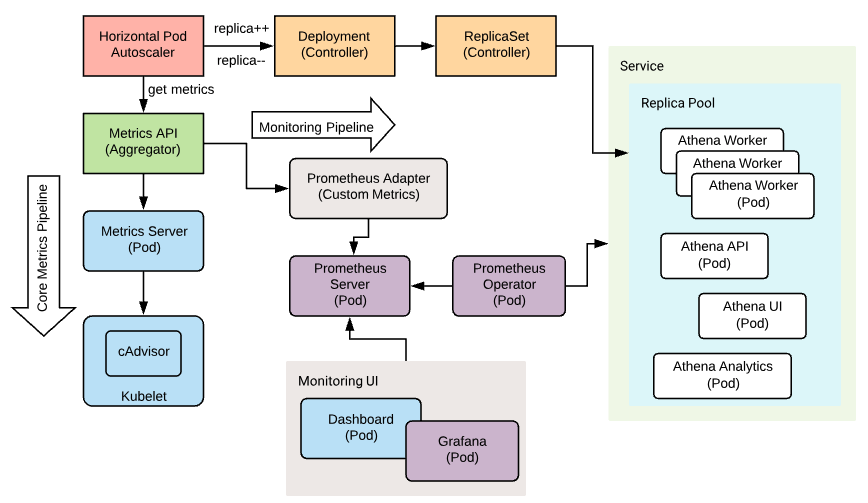
\includegraphics[width=0.7\paperwidth]{Figures/KUBE_monitoring}
\decoRule
\caption[Kubernetes Cluster: HPA and Monitoring for ATHENA]{Kubernetes Cluster: HPA and Monitoring for ATHENA}
\label{fig:kubeMonitAthena}
\end{figure}

Kubernetes Custom Metrics API along with the API Aggregation Layer make it possible for monitoring systems like Prometheus to expose application-specific metrics to the HPA controller. For Spring Boot application like ATHENA API service, it is relatively straight forward to expose metrics on JVM stats, embedded Tomcat (HTTP Requests/Responses traffic load) and any application-specific metrics (e.g. workload and number of Jobs in queue) using Actuator\footnote{\url{https://docs.spring.io/spring-boot/docs/current/reference/html/production-ready.html}} and Micrometer\footnote{\url{http://micrometer.io}}. 
\begin{small}
\begin{lcverbatim}
curl -s https://athena-dev.eresearch.unimelb.edu.au/prometheus
# HELP jvm_memory_used_bytes The amount of used memory
# TYPE jvm_memory_used_bytes gauge
jvm_memory_used_bytes{area="heap",id="PS Survivor Space",} 2.3983848E7
jvm_memory_used_bytes{area="heap",id="PS Old Gen",} 1.11927144E8
jvm_memory_used_bytes{area="heap",id="PS Eden Space",} 7.72185792E8
(scrap)
# HELP http_server_requests_duration_seconds Timer of servlet request
# TYPE http_server_requests_duration_seconds summary
http_server_requests_duration_seconds_count{method="GET",uri="/login",} 101.0
http_server_requests_duration_seconds_sum{method="GET",uri="/login",} 0.8731 218.975
(scrap)
\end{lcverbatim}
\end{small}


\newpage

\noindent \textbf{HPA Autoscaling Algorithm:} \quad Based on \parencite{kubeDoc}, the HPA implementation of autoscaling algorithm works as follow.

\begin{enumerate}
\item Implemented as a \textbf{Control Loop} - 30 seconds by default, configurable.
\item Periodically queries Pods to collects their CPU utilization
\item Compares the arithmetic mean of the Pods' CPU utilization with the target.
\item Adjusts the replicas of the Scale if needed to match the target, preserving condition: 
	\begin{itemize}
	\item MinReplicas <= Replicas <= MaxReplicas
	\item CPUUtilization (C) = recent CPU usage of a Pod (average across the last 1 minute)  / CPU requested by the Pod (\textit{spec.containers[].resources.requests.cpu}\footnote{\url{https://kubernetes.io/docs/tasks/configure-pod-container/assign-cpu-resource/}})
	\item TargetNumOfPods = ceil(sum(CurrentPodsCPUUtilization) / TargetCPUUtilizationPercentage (T))
	\[ TargetNumOfPods = \left \lceil \left ( \sum_{n=1}^{n} C_{n}  \right )  / T  \right \rceil \]
	\end{itemize}

\item Scale-up can only happen if there was no rescaling within the last 3 minutes. Due to temporarily CPU fluctuation during start/stop.
\item Scale-down will wait for 5 minutes from the last rescaling. Due to temporarily CPU fluctuation during start/stop.
\item Any scaling will only be made if: avg(CurrentPodsConsumption) / TargetCPUUtilizationPercentage drops below 0.9 or increases above 1.1 (10\% tolerance).
\end{enumerate}

\noindent \parencite{kubeDoc} states that algorithm approach has two benefits:
\begin{itemize}
\item Autoscaler works in a conservative way in such that increasing rapidly the number of Pods is important when user load is deteced. However, lowering the number of pods is not that urgent.
\item Autoscaler avoids thrashing, i.e. it prevents rapid execution of conflicting decision if the load is not stable.
\end{itemize}


%% OpenStack node scaling

\newpage

\section{Result and Finding}

Though Kubernetes is complex system to master thoroughly, when in operation, it is found that a very robust and flexible system. There also observable notice in overhead such as service proxies network layer. 

During the experimental runs, it is noticed that the auto-scaler doesn't react immediately to usage spikes. By default the metrics synchronisation happens once every 30 seconds and scaling up/down can only happen if there was no rescaling within the last 3-5 minutes. In this way, the HPA prevents rapid execution of conflicting decisions (oscillation). 

It is also found that auto-scaling based on observed CPU utilisation alone is not sufficient enough for ATHENA worker, due to the dynamic of how the simulation would run: \emph{simulation alone} or \emph{simulation + optimisation algorithm}. CPU utilisation scaling works better with optimisation algorithm on. However, simulation run alone with Monte Carlo job executed really quick. Therefore, it missed the scaling observation period delay time and consequently, it missed the HPA replication trigger cycle and there was only 1 worker Pod instance working on jobs. This can be tune accordingly to the target threshold and CPU utilisation feedback control loop, however, it is still not a perfect solution. In addition of CPU utilisation, observing job queue metrics should be implemented for a better work load balancing.

Figure~\ref{fig:kubeAthenaArch} depicts the architectural view of ATHENA deployment with Kubernetes cluster. Docker Registry is a container image registry hosted using Nexus repository manager.

\begin{figure}[H]
\centering
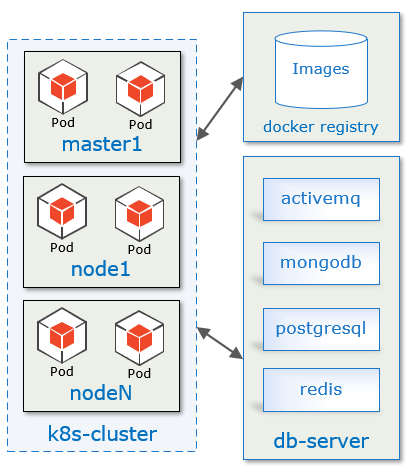
\includegraphics[width=0.4\paperwidth]{Figures/ATHENA_Kube_cluster}
\decoRule
\caption[Kubernetes Cluster for ATHENA Deployment: Architecture]{Kubernetes Cluster for ATHENA Deployment: Architecture}
\label{fig:kubeAthenaArch}
\end{figure}

Figure~\ref{fig:kubeAthenaTerm} shows the terminal screenshot of Kubernetes cluster up and running the ATHENA software stack. And Figure~\ref{fig:kubeAthenaGraf} shows the screenshot of Grafana\footnote{\url{https://grafana.com}} monitoring dashboard for observing  auto-scaling of ATHENA worker -- where the Replica trend shows the discrete steps of worker Pods scaling up/down, during a simulation run.

\begin{figure}[H]
\centering
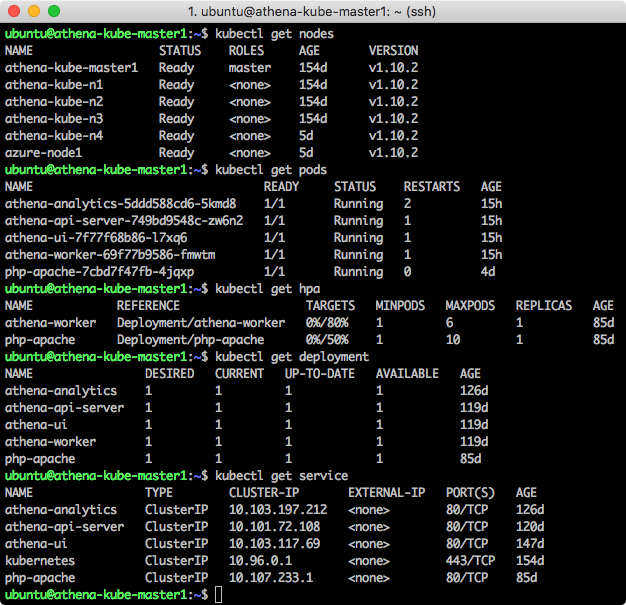
\includegraphics[width=0.6\paperwidth]{Figures/KUBE_ATHENA_term_long}
\decoRule
\caption[Kubernetes Cluster for ATHENA Deployment: Terminal]{Kubernetes Cluster for ATHENA Deployment: Terminal}
\label{fig:kubeAthenaTerm}
\end{figure}

\begin{figure}[H]
\centering
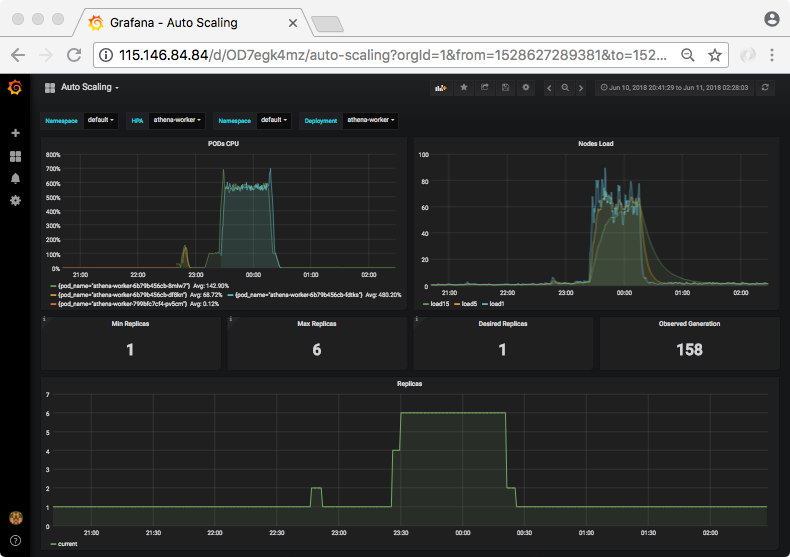
\includegraphics[width=0.6\paperwidth]{Figures/KUBE_ATHENA_grafana_autoscale_dash}
\decoRule
\caption[Kubernetes Cluster for ATHENA Deployment: Grafana]{Kubernetes Cluster for ATHENA Deployment: Grafana}
\label{fig:kubeAthenaGraf}
\end{figure}


Figure~\ref{fig:kubeAthenaProm} shows the screenshot of the Prometheus dashboard along with the Prometheus query and result graphing from Prometheus time-series database.

\begin{figure}[H]
\centering
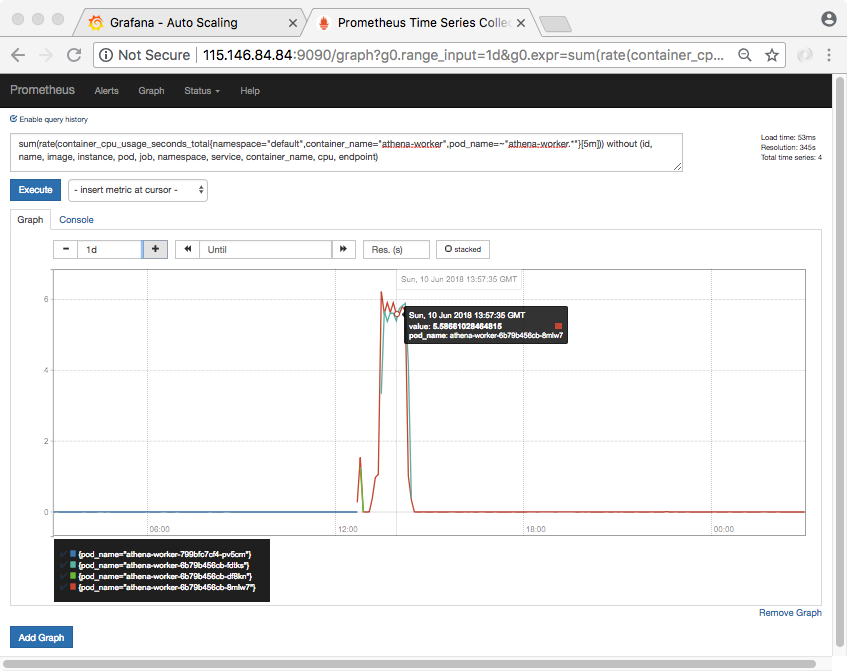
\includegraphics[width=0.7\paperwidth]{Figures/KUBE_ATHENA_prometheus}
\decoRule
\caption[Kubernetes Cluster for ATHENA Deployment: Prometheus]{Kubernetes Cluster for ATHENA Deployment: Prometheus}
\label{fig:kubeAthenaProm}
\end{figure}

The following is an example of Prometheus query that summing over
\\
\verb|container_cpu_usage_seconds_total| metrics at rate of 5 minutes averaging on all ATHENA worker Pods.

\begin{small}
\begin{lcverbatim}
sum(rate(container_cpu_usage_seconds_total{namespace="default",\
	container_name="athena-worker",pod_name=~"athena-worker.*"}[5m])) \
	without (id, name, image, instance, pod, job, namespace, service, \
	container_name, cpu, endpoint)
\end{lcverbatim}
\end{small}

The following is an example of Prometheus query that find the maximum of 
\\
\verb|kube_hpa_status_current_replicas| metrics -- the current max replica created by the HPA controller.

\begin{small}
\begin{lcverbatim}
max(kube_hpa_status_current_replicas{hpa="athena-worker",namespace="default"}) \
	without (instance, pod)
\end{lcverbatim}
\end{small}

